\documentclass{article}

\PassOptionsToPackage{numbers, compress}{natbib}










\newcommand{\theHalgorithm}{\arabic{algorithm}}
\usepackage{arxiv}
\usepackage[utf8]{inputenc} \usepackage[T1]{fontenc}    \usepackage{hyperref}       \usepackage{url}            \usepackage{booktabs}       \usepackage{amsfonts}       \usepackage{nicefrac}       \usepackage{microtype}      \usepackage{url}
\usepackage{graphicx}
\usepackage{algorithm}
\usepackage{algcompatible}
\usepackage{amsfonts}
\usepackage{amssymb}
\usepackage{amsthm}
\usepackage{amsmath}
\usepackage{bbm}
\usepackage{float}
\usepackage[font={rm,md,up}]{subfig}
\usepackage{caption,stackengine}
\usepackage{ragged2e}
\usepackage{tikz}
\usetikzlibrary{positioning}
\usetikzlibrary{arrows.meta}
\usepackage{multirow}
\usepackage{arydshln}

\makeatletter
\newcommand\footnoteref[1]{\protected@xdef\@thefnmark{\ref{#1}}\@footnotemark}
\makeatother

\tikzset{
  >={Latex[width=1mm,length=2mm]}
}

\tikzset{every picture/.style={line width=0.75pt}} 

\newcommand{\WRP}{\par\qquad\qquad\enspace}
\DeclareMathOperator*{\argmin}{argmin}

\title{Generalizing to unseen domains via distribution matching}



\author{Isabela Albuquerque\textsuperscript{1,}\thanks{Correspondence to \texttt{isabelamcalbuquerque@gmail.com}} , Jo\~ao Monteiro\textsuperscript{1}, Mohammad Darvishi\textsuperscript{2}, \textbf{Tiago H. Falk\textsuperscript{1}, Ioannis Mitliagkas\textsuperscript{3}}   
\\
\textsuperscript{1}INRS-EMT, Universit\'e du Qu\'ebec\\
\textsuperscript{2} Fauber Lab, Universit\'e de Montr\'eal \\ 
\textsuperscript{3}Mila \& DIRO, Universit\'e de Montr\'eal} 

\begin{document}

\maketitle

\begin{abstract}






Supervised learning results typically rely on assumptions of i.i.d. data. Unfortunately, those assumptions are commonly violated in practice. In this work, we tackle this problem by focusing on domain generalization: a formalization where the data generating process at test time may yield samples from never-before-seen domains (distributions).
Our work relies on a simple lemma: by minimizing a notion of discrepancy between all pairs from a set of given domains, we also minimize the discrepancy between any pairs of mixtures of domains. Using this result, we derive a generalization bound for our setting. We then show that low risk over unseen domains can be achieved by representing the data in a space where (i) the training distributions are indistinguishable, and (ii) relevant information for the task at hand is preserved. Minimizing the terms in our bound yields an adversarial formulation which estimates and minimizes pairwise discrepancies.
We validate our proposed strategy on standard domain generalization benchmarks, outperforming a number of recently introduced methods.
Notably, we tackle a real-world application where the underlying data corresponds to multi-channel electroencephalography time series from different subjects, each considered as a distinct domain.




\end{abstract}

\section{Introduction}

The main assumption within the empirical risk minimization framework is that all examples used for training and testing predictors are independently drawn from a fixed distribution, i.e. the i.i.d. assumption. A number of generalization guarantees were derived upon that assumption and those results induced several algorithms for the solution of supervised learning problems. However, important limitations in this setting can be highlighted: (i) the i.i.d. property is \emph{unverifiable} \cite{langford2005tutorial} given that one doesn't have access to the data distribution, and (ii) it doesn't account for distribution shifts, and those often occur in practice. Representative examples of such distribution shifts include changes in data acquisition conditions such as illumination in images for object segmentation, or new data sources such as unseen speakers when performing speech recognition. \\

A number of alternative settings was then introduced in order to better cope with more realistic cases. Risk minimization under the \emph{domain adaptation} setting, for instance, relaxes part of the i.i.d. assumption by allowing a source distribution (or domain)\footnote{We use the terms \textit{domain}, \textit{data distribution}, and \textit{data source} interchangeably throughout the text.} as well as a different target distribution observed at test time. Generalization results for this setting introduced in \cite{ben2007analysis} thus showed the generalization gap in terms of risk difference across the two considered distributions for a fixed predictor is upper bounded by a notion of distance measured between the training and testing domains. While less restrictive than the previous setting, the domain adaptation case is still limited in that only that pair of distributions is expected to yield low risk, and shifts beyond those domains will likely induce poor performance. Moreover, algorithms devised for this setting rely on access at training time to an unlabeled sample from the target distribution so that representations can be learned inducing invariance across train and target domains \cite{ganin2016domain}, which is further limiting considering practical cases, e.g. a speech recognition service cannot be trained on data obtained from every new speaker it observes.

A more general setting is often referred to as \textit{domain generalization} \cite{muandet2013domain}. In that case, it is assumed a set of distributions over the data is available at training time. At test time, however, both those observed distributions as well as unseen novel domains might appear, and a low risk is expected regardless of the underlying domain. More importantly, unlike domain adaptation settings in which the goal is to find a representation that aligns training data distributions with a specific target domain, \emph{domain generalization strategies aim at finding a representation space that yields good performance on novel distributions, unknown at training time.} Recent work on domain generalization has included the use of data augmentation \cite{shankar2018generalizing, volpi2018generalizing} at training time, meta-learning to simulate domain shift \cite{li2018learning}, adding a self-supervised task to encourage an encoder to learn robust representations \cite{carlucci2019domain}, learning domain-invariant representations \cite{li2018deep}, among other approaches.

In this contribution, we tackle the briefly described domain generalization setting. We first argue and prove that, given a set of distributions over data, if the distances measured between any pair of such distributions is small, so is the distance between mixtures obtained from the same set. That result yields a generalization guarantee to any distribution on the neighborhood of the ``convex hull''\footnote{i.e. the set of all mixtures obtained from given distributions.} defined by the set of domains we started with. Inspired by that, we define an approach so that an encoder is enforced to map the data to a space where domain-dependent cues are filtered away while relevant information to the task of interest is conserved. While doing so, no data from test distributions is required, \emph{which is a major advantage compared to more traditional domain adaptation settings} that target a specific distribution represented at training time through an unlabeled sample.

We summarize our contributions in the following:
\begin{itemize}
    \item We introduce a set of assumptions on the data generating process tailored to the domain generalization setting which we argue are much more general than standard i.i.d requirements and more likely to hold in practice, i.e. given a data sample, it is more likely that our assumptions will hold compared to the more restrictive i.i.d. property;
    \item We prove a generalization bound for the risk over unseen domains and show generalization can be expected for domains on the neighborhood of a notion of convex hull of distributions observed at training time;
    \item Aiming to minimize the bound introduced, we devise an adversarial approach so that pairwise domain divergences are estimated and minimized. In order to do so, several practical improvements are performed on top of previously introduced approaches for domain adaption including the use of random projections prior to domains discriminators. \end{itemize}

The remainder of this paper is organized as follows: In Section \ref{sec:background} we discuss past results which will be used in this work. In section \ref{sec:method} we define the domain generalization setting and present our main results as well as the resulting algorithm. Section \ref{sec:res} provides the experiments description and the respective results. Section \ref{sec:rel_work} discusses related work while conclusions are drawn in Section \ref{sec:conc} along with future directions.

\section{Background}\label{sec:background}
Let the data be represented by , while labels are given by , which would be  in the binary case, for instance. Examples correspond to a pair , such that , and  is a deterministic labeling function. 

A domain is defined as a tuple  where  corresponds to a probability distribution over . Moreover, we define a mapping , such that , where  is a set of candidate hypothesis, and finally define the risk  associated with a given hypothesis  on domain  as:

where the loss  quantifies how different  is from the true labeling function  for a given data instance .









\subsection{Generalization guarantees for domain adaptation} 
We now state results from the domain adaptation literature which are relevant for this work. 
The discussion in \cite{ben2010theory} established the theoretical foundations for studying the cross-domain generalization properties for domain adaptation problems. Based on the \emph{covariate shift assumption}, which considers that the labeling function is the same across domains (i.e. while  can change,  is fixed) they showed that, given a source domain  and target domain , the risk of a given hypothesis  on the target is bounded by:

where  corresponds to the minimal total risk over both domains which can be achieved within a given hypothesis class . The term  corresponds to the -divergence introduced in \cite{kifer2004detecting} and defined is as follows: 

As discussed in \cite{ben2007analysis}, an estimate of  can be directly computed from the error of a binary classifier trained to distinguish domains.

In \cite{zhao2018adversarial}, an extension of the bound above was presented for the case where multiple source domains are available at training time. Given  source domains , , and a mixture of the source domains , the risk  on the target domain is bounded by: 

where  is the minimum total risk, i.e. the sum of the risks measured on the target and the mixture of the sources, one can get within the considered hypothesis class, and the set  of mixture coefficients is such that .

\section{Learning domain agnostic representations for domain generalization}\label{sec:method}



\subsection{Formalizing domain generalization}

We start by defining a set of assumptions we introduce over the data generating process considering the domain generalization case as well as the notion of risk we are concerned with. We then define , referred to as meta-distribution, corresponding to a probability distribution over a countable set of possible domains. Under this view, a query for a data example consists of: (i) sampling a domain from the meta-distribution, and (ii) sampling a data point according to that particular domain. Such process is repeated  times so as to yield a training sample . We remark the described model of data generating processes is sufficiently general so as to include the i.i.d. case (the meta-distribution yields a single domain) as well as the domain adaptation setting (if two domains are allowed), but further supports several other cases where multiple domains exist.

\begin{figure}[h]
\centering
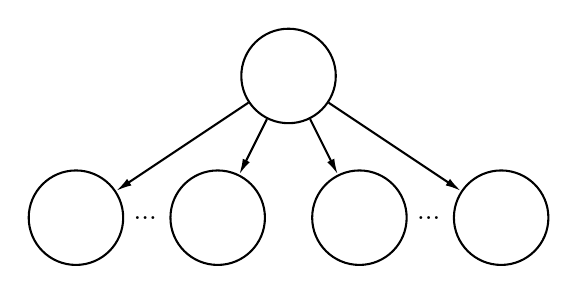
\begin{tikzpicture}[->, level/.style={sibling distance = 2cm/#1,
  level distance = 2cm}, state/.style={circle, draw, minimum size=1.2cm}, x=0.45pt,y=0.4pt,yscale=0.9,xscale=0.9]
\node[circle, state, draw](A){\Large{}}
  child{node[circle, state, draw](B){}}
child{node[circle, state, draw](C){}}
  child{node[circle, state, draw](D){}}
  child{node[circle, state, draw](E){}};
\node[left = of C, xshift=0.97cm] {...};
\node[left = of E, xshift=0.97cm] {...};
\end{tikzpicture}
\caption{Illustration of the meta-distribution  composed by the source and unseen domains.}
\label{fig:meta_dist}
\end{figure}
\noindent Figure \ref{fig:meta_dist} illustrates the general model of data generating processes by representing the meta-distribution along with possible domains. We remark that, once a finite train sample is collected, a set of  domains is observed. Each distribution , , in such set will be referred to as source domain. At test time however, drawing samples from  might yield data distributed according to new unseen domains. We then introduce extra notation and represent the set of possible domains unobserved while train data is acquired by , . 


\noindent We proceed and define a risk minimization framework similar to that corresponding to the i.i.d. setting: find the predictor  that minimizes the meta-risk  defined as follows: 

However, within the domain generalization setting, no information regarding possible test distributions is available at training time, which renders estimating  uninformative for a practical number of source domains. Moreover, we argue that no-free-lunch type of impossibility results may be used to conclude that it is impossible to generalize to any possible unknown distribution\footnote{For a fixed hypothesis, one can always define a distribution yielding high risk.}, so that one must assume something about the test domains in order to enable generalization. In the following results, we tackle that issue and introduce generalization guarantees for a particular set of domains lying close to the set of mixtures of \emph{source distributions}, i.e. those observed once train data is collected
\cite{hoffman2018algorithms}.

\subsection{Matching distributions in the convex hull}
Let a set  of source domains such that  be denoted by , . The convex hull  of  is defined as the set of mixture distributions given by: .  
The following proposition shows that for any pair of domains such that , the -divergence between  and  is upper-bounded by the largest -divergence measured between elements of .

\textbf{Proposition 1} \textit{(Bounding the -divergence between domains in the convex hull). Let . The following inequality holds for the -divergence between any pair of domains }:

\textit{Proof.} C.f. supplementary material. 

We thus argue that if one minimizes the maximum pairwise -divergence between source domains, which can be achieved by an encoding process that filters away domain discriminative cues, the -divergence between any two domains in  also decreases. 

\subsection{Generalizing to unseen domains}
Now we turn our attention to the set of unseen distributions , , i.e. those in the support of the meta-distribution but not observed within the training sample. We further introduce , the element of  which is closest to , i.e.   is given by . Based on Proposition 1, we derive a generalization bound for the risk  in terms of  and :

\textbf{Proposition 2} \textit{(Generalization to unseen domains). Let . Given the previous setup and assumptions, the following inequality holds for the risk ,  for \textbf{any} domain }:

\textit{where  is the minimum sum of the risks achieved by some  on  and .}

\textit{Proof.} C.f. supplementary material.

The result discussed on the above can be used to define algorithms relying solely on source data, \emph{unlike domain adaptation approaches}. While the total source risk can be minimized as usual,  can be minimized by encoding source data to a space where source domains are hard to distinguish. 

We further highlight that such results also provide insights regarding the importance of acquiring diverse datasets in practice when targeting  domain generalization. The more diverse a dataset is regarding the number of domains present at training time, more likely it is that an unseen distribution lies within the convex hull of the source domains. In this case,  and the bound stated in Proposition 2 is tighter. Therefore, not only the amount of data is important to achieve better  generalization on unseen domains, but also the diversity of the training data is crucial. Another practical aspect worth remarking is that, even though our domain generalization setting is more general than ERM, Proposition 2 suggests that source domain labels should also be available, since they are required to estimate , which is not the case for ERM. However, collecting domain labels is inherent to the data acquisition procedure for several tasks and commonly available as meta-data in cases such as, for example, speech recognition, where different speakers or channels can be viewed as different domains.

\subsection{Practical contributions}
Motivated by the previous results, we propose to estimate and minimize  along with the risks over the train sample. We thus aim at learning an encoder , where  preserves information relevant for separating classes, while removing domain-specific cues in such a way that it is harder to distinguish examples from different domains in comparison to the original space . 

\textbf{Efficiently estimating :} Previous work on domain adaptation introduced strategies based on minimizing the empirical -divergence between sources and a given target domain \cite{ganin2016domain, zhao2018adversarial}. Instead, as per the discussion following Proposition 2, the domain generalization setting requires estimating pairwise -divergences across all available sources, not considering target data of any sort. Naively extending previous methods to our case would require  estimators, which is unpractical given real-world cases where several source domains are available. We thus propose to use {\em one-vs-all} classifiers. In this case, there is one domain discriminator per source domain and the -th discriminator estimates\footnote{\label{fn:supmat}See supplementary material for details.} , and improves the method to a number of -divergence estimators linear on .

\textbf{Training:} 
The proposed approach contains three main modules: an encoder  with parameters , a task classifier  with parameters , and a set of -divergence estimators  with parameters , . Intuitively,  attempts to minimize a classification loss  (standard cross-entropy in our case) and empirical -divergences, which is achieved through the maximization of domain discrimination losses, denominated . Each domain discriminator, on the other hand, aims at minimizing . The procedure for estimating , , and all 's can be thus formulated as the following multiplayer minimax game:   

where  corresponds to the task label for the example , and  is equal to 1 in case , or 0 otherwise. 
Training is carried out with alternate updates. A pseudocode describing the training procedure is presented in Algorithm \ref{pseudo_code}.

\begin{algorithm*}[h]
\caption{Generalizing to unseen Domains via Distribution Matching}\label{pseudo_code}
\begin{algorithmic}[1]
\STATE Requires: classifier and encoder learning rate (), domain discriminators learning rate (), scaling (), mini-batch size ().
\STATE Initialize , ,  as , , . 
\FOR { number of iterations}
\STATE Sample one mini-batch from each source domain 
\STATE \texttt{ Update domain discriminators}
\FOR {}
\STATE 
\ENDFOR
\STATE \texttt{ Update task classifier}
\STATE 
\STATE \texttt{ Update encoder}
\STATE   \\ 

\ENDFOR
\end{algorithmic}
\end{algorithm*}

We empirically found it helpful to augment our domain generalization approach with strategies for stabilizing the training of generative adversarial networks with multiple discriminators \cite{neyshabur2017stabilizing, albuquerque2019multi}. A random projection layer is then introduced in the input of each domain discriminator with the goal of making examples from different distributions harder to be distinguished, and the negative log hypervolume is used instead of the summation in the game represented in (\ref{eq:game})\footnoteref{fn:supmat}. We refer to the proposed approach as G2DM (\textbf{G}eneralizing to unseen \textbf{D}omains via \textbf{D}istribution \textbf{M}atching).

\textbf{Differences to multi-source domain adaptation:} We further remark the differences between G2DM and previous adversarial approaches which are often employed in domain adaptation. Essentially, G2DM compares examples \emph{only from source domains} to learn domain-agnostic representations, i.e. there is no notion of target distribution. Other settings such as \cite{zhao2018adversarial} are more restricted in that a particular distribution is targeted and data from that distribution is required, besides the source data we use in our case. Moreover, those approaches do not aim at matching source distributions and only consider -divergences computed between each source domain and the given target. In the case of G2DM on the other hand, the goal is to match source domain distributions to decrease , and thus only pairwise discrepancies between training domains are considered. 

\section{Experiments}\label{sec:res}
Our empirical evaluation aims to answer the following questions: (i) Can we do better than standard ERM under i.i.d. assumptions by using information of source domains only? (ii) where does G2DM's performance stand in comparison to previous work? (iii) is G2DM indeed enforcing distribution matching? (iv) what is the effect on the resulting performance of employing different stopping criteria? We start the investigation performing experiments on two domain generalization benchmarks (VLCS \cite{fang2013unbiased} and PACS \cite{li2017deeper}) which consist of object recognition tasks. We then evaluate G2DM on a real-world task that involves classifying electroencephalography (EEG) time series for affective state prediction. Additionally, in the supplementary material we provide results showing the impact of the random projection layer size and the number of source domains on final performance.

\subsection{VLCS and PACS benchmarks}


The VLCS benchmark is composed of 5 overlapping classes of objects obtained from the VOC2007 \cite{everingham2010pascal}, LabelMe \cite{russell2008labelme}, Caltech-101 \cite{griffin2007caltech}, and SUN \cite{choi2010exploiting} datasets. The object recognition benchmark referred to as PACS, in turn, consists of images distributed into 7 classes originated from four different datasets: Photo (P), Art painting (A), Cartoon (C), and Sketch (S). Details regarding each benchmark can be found in the supplementary material. We compare the performance of our proposed approach with a model trained with ERM over all source domains with no mechanisms to enforce domain generalization. Moreover, we consider the recently introduced invariant risk minimization (IRM) strategy \cite{arjovsky2019invariant} and include results reported in the literature achieved by Epi-FCR \cite{li2019episodic}, JiGen \cite{carlucci2019domain} along with the ERM results they provided (referred to as ERM-JiGen), and MMD-AAE \cite{li2018domain}. Finally, the adaptation of DANN for domain generalization reported in \cite{li2019episodic} was also considered. All such methods have an encoder implemented as the convolutional stack of AlexNet \cite{krizhevsky2012imagenet} and the weights are initialized from the pre-trained model on ImageNet \cite{deng2009imagenet}. Further implementation details necessary for reproducing the results reported herein can be found in the supplementary material.


In Tables \ref{res:tab_vlcs} and \ref{res:tab_pacs}, we report the average best accuracy across three runs with different random seeds on the test partition of the unseen domain under a leave-one-domain-out validation scheme. Results show that G2DM outperforms ERM in terms of average performance across the unseen domains for both benchmarks, and supports the claim that leveraging source domain information as done by G2DM provides an improvement on generalization to unseen distributions in comparison to simply considering the i.i.d. requirement is satisfied. G2DM further presented better average performance when compared to our implementation of IRM, as well as results from other methods previously reported in the literature. We finally highlight that G2DM showed an improvement in performance in more challenging domains \cite{li2017deeper} such as LabelMe and Sketch. 

\vspace{0.3cm}
\begin{minipage}{\textwidth}
\begin{minipage}[t]{0.49\textwidth}
\captionof{table}{Classification accuracy () for models trained considering leave-one-domain-out validation on the VLCS benchmark.}
\centering
\resizebox{0.9\columnwidth}{!}{
\begin{tabular}{c|cccc|c}
\hline
Unseen domain () & V     & L     & C     & S     & Average \\ \hline
DANN \cite{li2019episodic}                 & 66.40 & 64.00 & 92.60 & 63.60 & 71.70   \\
MMD-AAE \cite{li2018domain}              & 67.70 & 62.60 & 94.40 & 64.40 & 72.28   \\
Epi-FCR \cite{li2019episodic}              & 67.10 & 64.30 & 94.10 & 65.90 & 72.90   \\
JiGen \cite{carlucci2019domain}                & 70.62 & 60.90 & 96.93 & 64.30 & 73.19   \\
ERM - JiGen \cite{carlucci2019domain}          & 71.96 & 59.18 & 96.93 & 62.57 & 72.66   \\
IRM                   & 72.16 & 62.36 & \textbf{98.35} & 67.82 & 75.17   \\
ERM                   & \textbf{73.44} & 60.44 & 97.88 & 67.92 & 74.92   \\ \hline
G2DM                  & 71.14 & \textbf{67.63} & 95.52 & \textbf{69.37} & \textbf{75.92}   \\ \hline
\end{tabular}}
\label{res:tab_vlcs}
\end{minipage}
\hfill
\begin{minipage}[t]{0.49\textwidth}
\centering
\captionof{table}{Classification accuracy () for models trained considering leave-one-domain-out validation on the PACS benchmark.}
\resizebox{\columnwidth}{!}{
\begin{tabular}{c|cccc|c}
\hline
Unseen domain ()     & P     & A     & C     & S     & Average \\ \hline

DANN \cite{li2019episodic}      & 88.10  & 63.20  & 67.50  & 57.00    & 69.00      \\
Epi-FCR \cite{li2019episodic}   & 86.10  & 64.70  & 72.30  & 65.00 & 72.00      \\
JiGen \cite{carlucci2019domain}     & 89.00    & \textbf{67.63} & 71.71 & 65.18 & 73.38   \\
ERM - JiGen \cite{carlucci2019domain} & 89.98 & 66.68 & 69.41 & 60.02 & 71.52   \\
IRM        & 89.97 & 64.84 & 71.16  & 63.63 & 72.39         \\
ERM         & \textbf{90.02} & 64.86 & 70.18 & 61.40  & 71.61   \\ \hline
G2DM       & 88.12 & 66.60  & \textbf{73.36} & 
\textbf{66.19} & \textbf{73.55}   \\ \hline
\end{tabular}
}
\label{res:tab_pacs}

\end{minipage}
\end{minipage}

\vspace{0.3cm}
\subsubsection{Estimating pairwise -divergences} We investigate whether cross-domain -divergences are being in fact reduced by G2DM. We use ERM as a baseline for comparison since it does not include any mechanism to enforce distribution matching. We estimate -divergences by computing the proxy pairwise -distance \cite{ben2007analysis} for each pair of domains on the PACS benchmark. Classifiers are trained on top of the representations  obtained with ERM and G2DM. We show in Figures \ref{fig:a_dist} the differences in estimated discrepancies between ERM and G2DM for each unseen domain. Each entry corresponds to a pair of domains indicated in the row and the column and positive values indicate that G2DM \emph{decreased} the corresponding pairwise -distance in comparison to ERM. Notice that the diagonals are left blank as we do not compute the domain classification accuracy between the same domains. We observe that apart from the case where Photo is the unseen domain, G2DM was able to better match most of the source domains, thus yielding a smaller  which favours generalization. Interestingly, we also noticed that the estimated pairwise -divergence between the unseen domain and sources also decreased in most of the cases even though G2DM did not have access to data from the unseen domain at training time to explicitly match those distributions. This effect is explained by the fact that the -divergence satisfies the triangle inequality (c.f. Eq. \ref{eq:triangle} in the supplementary material), which can be used to show that an upper-bound for the discrepancy between the unseen domain and any source gets tighter once  decreases. 
\begin{figure}[h]
	\centering
	\subfloat[photo][Photo.]{\includegraphics[width=0.24\textwidth]{h_dist/photo_diff_disparity_hmap_pink.png}}
	\;
	\subfloat[art][Art.]{\includegraphics[width=0.24\textwidth]{h_dist/art_diff_disparity_hmap_pink.png}}
    \;
	\subfloat[cartoon][Cartoon.]{\includegraphics[width=0.24\textwidth]{h_dist/cartoon_diff_disparity_hmap_pink.png}}
	\;
	\subfloat[sketch][Sketch.]{\includegraphics[width=0.24\textwidth]{h_dist/sketch_diff_disparity_hmap_pink.png}}
	\caption{Differences between estimated pairwise -divergences under ERM and G2DM on PACS (captions denote unseen domains). Higher values indicate that G2DM better matched domains. Overall, G2DM is able to decrease pairwise discrepancies.}
	\label{fig:a_dist}
 \end{figure}



\subsubsection{Domain generalization in practical scenarios} Results of previous experiments correspond to an optimistic scenario where target data is available for at least selecting the best performing model. This is not the case in practice since varying target distributions might appear. In Table \ref{tab:stop_crit}, we compare results obtained further considering stopping criteria that only use information from the source domains, such as validation accuracy on the source domains and training task loss. For comparison, we also present the performance reported by \cite{li2018deep} for CIDDG, since a stopping criterion using solely data from source domains was employed in that case. We notice that, when using the task loss as stopping criterion, our strategy outperforms CIDDG for almost all domains while its performance severely degrades when Sketch is the unseen domain. As an alternative to AlexNet, we further evaluate the performance of the proposed approach using the convolutional stack of a ResNet-18 \cite{he2016deep}, since it has shown promising results in recent work \cite{carlucci2019domain}.
We compare our approach with JiGen\footnote{\label{fn:jigen}Results are generated using JiGen authors' source code (\url{https://github.com/fmcarlucci/JigenDG}).} adopting the same previous stopping criteria for both methods. We further report in Table \ref{tab:stop_crit} the performance obtained by JiGen as reported in \cite{carlucci2019domain} although it is unclear which stopping criteria were adopted for that case. We observe that replacing AlexNet by ResNet-18 yields a more stable average performance across stopping criteria. Based mostly on the results obtained with AlexNet, we remark that different criteria might be too optimistic/pessimistic, and as such, one practical recommendation we can draw from our results is that the best methodology to be adopted when studying domain generalization strategies is to \emph{report their performance across different stopping criteria}.
\subsection{Real-world case: Affective state prediction from multi-variate time-series}




We proceed to evaluate the proposed approach beyond domain generalization benchmarks. The goal of the selected task is to perform affective state estimation based on EEG signals from multiple subjects. EEG is a modality known to present high variability across different individuals given the same stimuli due to factors such as anatomic and environment variations \cite{wu2015reducing}. Therefore, since it cannot be assumed data from different individuals are identically distributed, this scenario consists in a challenging test bed for domain generalization approaches. We use the SEED dataset \cite{zheng2015investigating}, which is composed of 62-channel EEG signals from 15 participants. During the data collection, subjects are asked to rate video clips extracted from movies as positive, neutral, or negative. We follow \cite{li2018extracting} and use the architecture described in \cite{li2017targeting} for both G2DM and ERM. We consider each subject as a different domain and perform leave-one-subject-out evaluation. For each subject left out for testing, we use 10 out of remaining 14 domains for training and use the other 4 as validation data. Similarly to our previous experiments, for each test domain we perform 3 independent runs. We report in Table \ref{tab:seed_acc} the affective state prediction accuracy () averaged across all unseen subjects and runs. Under \textbf{source data validation}, the performance reported was computed on the epoch of highest accuracy on the source domains at the validation partition. The results under \textbf{semi-privileged} were obtained on the epoch of highest accuracy on the unseen subject. The comparison between G2DM and ERM shows that using G2DM to leverage domain information (which in this case comes with no additional effort at the data collection) yields an improvement in performance for both stopping criteria. 
We further report in Table \ref{tab:seed_acc} results obtained by domain adaptation strategies (DA). Such methods, reported in Table \ref{tab:seed_acc} under \textbf{privileged baselines}, are privileged in the sense that unlabeled data belonging to the target domain (unknown in our case) is used to adapt representations to yield subject-specific models. When comparing the DA strategies with our domain generalization (DG) approach, we remark that DG strategies aim to obtain domain-agnostic models, as opposed to DA methods which target a specific distribution. As such, one would expect DA approaches to achieve better performance than DG. However, we observe G2DM's performance to be on par or even better than some of the considered DA strategies. We conjecture a larger number of source domains available at training time would decrease the gap between DG and DA even further; i.e. it would be more likely that unseen domains are exactly represented in the convex hull of the sources yielding low  (c.f. Proposition 2).

\vspace{0.5cm}
\begin{minipage}{\textwidth}
\begin{minipage}[t]{0.6\textwidth}
\captionof{table}{Accuracy () on PACS with different stopping criteria.}
\resizebox{\columnwidth}{2.54cm}{
\begin{tabular}{ccccccc}
\hline
  Method & Criterion  & P     & A     & C     & S & Average    \\ \hline
                \multicolumn{7}{c}{\textbf{AlexNet}}                                         \\ \hline
CIDDG \cite{li2018deep}                 & \footnotesize{From \cite{li2018deep}}  & 78.65 & 62.70 & 69.73 & 64.45 & 68.88          \\  \hdashline
\multirow{3}{*}{G2DM} & Source acc.  & 85.33 & 57.76 & 69.71 & 49.45 & 65.56     \\
                      & Source loss & 87.37 & 66.70 & 70.26 & 50.98 & 68.82   \\
                      & Unseen acc. & 88.80 & 66.70 & 73.29 & 65.03 & 73.45 \\ \hline
\multicolumn{7}{c}{\textbf{ResNet-18}}                                                       \\ \hline
\multirow{4}{*}{JiGen \cite{carlucci2019domain}} & Source acc.  & 95.83 & 78.52 & 73.31 & 69.14 & 79.20 \\ 
                       & Source loss & 95.83 & 78.89 & 73.32 & 70.73 & 79.69 \\
                       & Unseen acc. & 96.11 & 79.56 & 74.25 & 71.00 & 80.23 \\
                       & \footnotesize{From \cite{carlucci2019domain}} & 96.03 & 79.42 & 75.25 & 71.35 & 80.51 \\  \hdashline
\multirow{3}{*}{G2DM} & Source acc.  & 93.70 & 79.22 & 76.34 & 75.14 & 81.10   \\
                      & Source loss & 93.75 & 77.78 & 75.54 & 77.58 & 81.16 \\
                      & Unseen acc. & 94.63 & 81.44 & 79.35 & 79.52 & 83.34   \\
                       \hline  


\end{tabular}
}
\label{tab:stop_crit}
\end{minipage}
\hspace{0.1cm}
\begin{minipage}[t]{0.38\textwidth}
\centering
\captionof{table}{Average accuracy () on the SEED dataset across 15 subjects. Privileged baselines have access to unseen domain data.}
\resizebox{\columnwidth}{!}{
\begin{tabular}{ccc}
\hline
                    Setting & Method & Average acc. ()  \\ \hline 
\multirow{5}{*}{DG} & \multicolumn{2}{c}{\textit{Source data validation}} \\ \cline{2-3}
                    & ERM  & 51.98           \\
                    & G2DM & \textbf{55.77}  \\ \cline{2-3}
                    & \multicolumn{2}{c}{\textit{Semi-privileged}} \\ \cline{2-3}
                    & ERM &  56.82  \\ 
                    & G2DM & \textbf{60.26}  \\ \hline
\multicolumn{3}{c}{\textit{Privileged baselines}} \\ \hline
\multirow{4}{*}{DA}   & DAN \cite{long2015learning,li2018extracting}  & 50.28                \\
                      & DANN \cite{ganin2016domain,li2018extracting} & 55.87                \\
                      & MDAN \cite{zhao2018adversarial,li2018extracting} & 56.65                \\
                      & MDMN \cite{li2018extracting} & 60.59                \\ \hline
\end{tabular}
}
\label{tab:seed_acc}
\end{minipage}
\end{minipage}
\vspace{0.2cm}
\section{Related work}\label{sec:rel_work}
In \cite{carlucci2019domain}, authors proposed to enforce generalization to unseen domains by adding a regularization term that depends on a self-supervised task. Other work proposed to enforce domain generalization with adversarial approaches. This is the case of CIDDG \cite{li2018deep}, where class-specific domain classifiers are employed to induce the encoder to learn representations where the mismatch between the labels conditional distributions is minimized. Moreover, MMD-AAE \cite{li2018domain}, proposed an approach that relies on an adversarial autoencoder and a maximum mean discrepancy penalty to remove domain-specific information. Recent approaches also proposed to simulate domain-shifts at training time by splitting the source domains into meta-train and meta-test sets \cite{li2018learning,balaji2018metareg,dou2019domain} or by proposing an episodic training approach as in Epi-FCR \cite{li2019episodic}. Previous work also included strategies based on learning domain-invariant representations \cite{muandet2013domain,arjovsky2019invariant}, data augmentation \cite{volpi2018generalizing,shankar2018generalizing}, and on decomposing the model's parameters into domain-agnostic and domain-specific components \cite{li2017deeper}.
Work on other settings with more restrictive assumptions than domain generalization are also related to our contribution. For example, recent work on multi-domain learning \cite{schoenauer2019multi}, a setting where multiple domains are available at training time and test data is drawn from the same distributions seen during training \cite{dredze2010multi}, also leveraged -divergence minimization to derive an adversarial approach.



\section{Conclusion}\label{sec:conc}






We tackled the domain generalization setting and showed generalization can be achieved in the neighborhood of the set of mixtures of distributions observed during training. Based on this result, we introduced G2DM, an efficient approach in yielding invariant representations across unseen distributions. Our method employs multiple one-vs-all domain discriminators such that pairwise divergences between source distributions are estimated and minimized at training time. We provide empirical evidence that making use of domain information enables a boost in performance compared to standard settings relying on i.i.d. requirements. Moreover, the introduced approach outperformed recent methods which also leverage domain labels. We further showed  such approach to yield strong results on a realistic setting, with performance comparable to privileged systems tailored to test distributions. In future work, we intend to investigate if the introduced assumptions on the data generating process can yield PAC-like results for domain complexity in a meta-distribution-agnostic fashion, i.e. we intend to assess questions such as: how many source domains are needed to guarantee low meta-risk with high probability?

















\bibliographystyle{IEEEtran}
\bibliography{references.bib}

\clearpage
\appendix
\section*{Supplementary Material}

\section{Proof of Proposition 1}
Consider two unseen domains,  and  on the convex-hull  of  source domains with support . Consider also  and 
The -divergence between  and  can be written as:

Using the triangle inequality, we can write:


Finally, using the sub-additivity of the :













Given  :



\section{Proof of Proposition 2}
Recall the result from \cite{zhao2018adversarial} for the multi-source domain adaptation setting (for the sake of clarity, stated here replacing the target domain by an unseen domain according to our notation):


Using the triangle inequality for the -divergence, we can bound the -divergence between an unseen domain  and a source domain ,    by:

where  is the -divergence between  and the convex-hull of the sources, i.e.  such that .

We can now choose each 's to correspond to the 's and re-write Eq. \ref{eq:bound_msda2} for an unseen domain  as



Using Eq. \ref{eq:triangle}, we can upper-bound  by , which gives  




\section{One-vs-all -divergence estimation}
We illustrate the estimation of -divergences using one-vs-all discriminators by considering an example in which 3 source domains are available. Consider samples of size  from  source domains which are available at training time. The loss  for the domain discriminator  accounting for estimating  and  can be written as:


 
where  represents a loss function (e.g. 0-1 loss) and each term accounts for the loss provided by examples from one domain. Splitting the first term in two parts and replacing the domain labels  by their corresponding values, we obtain:


The first two terms from Eq.\ref{eq:hdiv_decomp} account for  and the last two terms account for .

\section{Illustration}
\tikzset{every picture/.style={line width=0.75pt}} \begin{figure}[h]
\centering
\resizebox{0.4\columnwidth}{5cm}{

\begin{tikzpicture}[x=0.75pt,y=0.75pt,yscale=-1,xscale=1]

\draw  [fill={rgb, 255:red, 151; green, 221; blue, 204 }  ,fill opacity=1 ] (127,148) .. controls (127,143.58) and (130.58,140) .. (135,140) -- (210,140) .. controls (214.42,140) and (218,143.58) .. (218,148) -- (218,172) .. controls (218,176.42) and (214.42,180) .. (210,180) -- (135,180) .. controls (130.58,180) and (127,176.42) .. (127,172) -- cycle ;
\draw  [fill={rgb, 255:red, 151; green, 221; blue, 204 }  ,fill opacity=1 ] (135,158) .. controls (135,153.58) and (138.58,150) .. (143,150) -- (218,150) .. controls (222.42,150) and (226,153.58) .. (226,158) -- (226,182) .. controls (226,186.42) and (222.42,190) .. (218,190) -- (143,190) .. controls (138.58,190) and (135,186.42) .. (135,182) -- cycle ;
\draw  [fill={rgb, 255:red, 241; green, 161; blue, 226 }  ,fill opacity=1 ] (276,229.2) .. controls (276,224.67) and (279.67,221) .. (284.2,221) -- (380.8,221) .. controls (385.33,221) and (389,224.67) .. (389,229.2) -- (389,253.8) .. controls (389,258.33) and (385.33,262) .. (380.8,262) -- (284.2,262) .. controls (279.67,262) and (276,258.33) .. (276,253.8) -- cycle ;
\draw  [fill={rgb, 255:red, 158; green, 201; blue, 250 }  ,fill opacity=1 ] (285,59) .. controls (285,54.58) and (288.58,51) .. (293,51) -- (378,51) .. controls (382.42,51) and (386,54.58) .. (386,59) -- (386,83) .. controls (386,87.42) and (382.42,91) .. (378,91) -- (293,91) .. controls (288.58,91) and (285,87.42) .. (285,83) -- cycle ;
\draw (60,119) node  {\includegraphics[width=39pt,height=36pt]{art.png}};
\draw (56.5,185.5) node  {\includegraphics[width=33.75pt,height=30.75pt]{cartoon.png}};
\draw (57.5,251) node  {\includegraphics[width=39.75pt,height=34.5pt]{photo.png}};
\draw (495,244) node  {\includegraphics[width=39pt,height=36pt]{art.png}};
\draw (628.5,241.5) node  {\includegraphics[width=33.75pt,height=30.75pt]{cartoon.png}};
\draw (565.5,240) node  {\includegraphics[width=39.75pt,height=34.5pt]{photo.png}};
\draw  [color={rgb, 255:red, 144; green, 19; blue, 254 }  ,draw opacity=1 ][dash pattern={on 5.63pt off 4.5pt}][line width=1.5]  (460,215) -- (524,215) -- (524,269) -- (460,269) -- cycle ;
\draw  [color={rgb, 255:red, 208; green, 2; blue, 27 }  ,draw opacity=1 ][dash pattern={on 1.69pt off 2.76pt}][line width=1.5]  (534,215) -- (661,215) -- (661,269) -- (534,269) -- cycle ;
\draw (626,349) node  {\includegraphics[width=39pt,height=36pt]{art.png}};
\draw (494.5,351.5) node  {\includegraphics[width=33.75pt,height=30.75pt]{cartoon.png}};
\draw (566.5,348) node  {\includegraphics[width=39.75pt,height=34.5pt]{photo.png}};
\draw  [color={rgb, 255:red, 144; green, 19; blue, 254 }  ,draw opacity=1 ][dash pattern={on 5.63pt off 4.5pt}][line width=1.5]  (461,323) -- (525,323) -- (525,377) -- (461,377) -- cycle ;
\draw  [color={rgb, 255:red, 208; green, 2; blue, 27 }  ,draw opacity=1 ][dash pattern={on 1.69pt off 2.76pt}][line width=1.5]  (535,323) -- (662,323) -- (662,377) -- (535,377) -- cycle ;
\draw (573,457) node  {\includegraphics[width=39pt,height=36pt]{art.png}};
\draw (626.5,458.5) node  {\includegraphics[width=33.75pt,height=30.75pt]{cartoon.png}};
\draw (494.5,458) node  {\includegraphics[width=39.75pt,height=34.5pt]{photo.png}};
\draw  [color={rgb, 255:red, 144; green, 19; blue, 254 }  ,draw opacity=1 ][dash pattern={on 5.63pt off 4.5pt}][line width=1.5]  (462,431) -- (526,431) -- (526,485) -- (462,485) -- cycle ;
\draw  [color={rgb, 255:red, 208; green, 2; blue, 27 }  ,draw opacity=1 ][dash pattern={on 1.69pt off 2.76pt}][line width=1.5]  (536,431) -- (663,431) -- (663,485) -- (536,485) -- cycle ;
\draw [color={rgb, 255:red, 109; green, 109; blue, 109 }  ,draw opacity=1 ]   (98,165) -- (124,165) ;
\draw [shift={(126,165)}, rotate = 180] [color={rgb, 255:red, 109; green, 109; blue, 109 }  ,draw opacity=1 ][line width=0.75]    (10.93,-3.29) .. controls (6.95,-1.4) and (3.31,-0.3) .. (0,0) .. controls (3.31,0.3) and (6.95,1.4) .. (10.93,3.29)   ;

\draw [color={rgb, 255:red, 109; green, 109; blue, 109 }  ,draw opacity=1 ]   (233,180) -- (274.82,237.38) ;
\draw [shift={(276,239)}, rotate = 233.91] [color={rgb, 255:red, 109; green, 109; blue, 109 }  ,draw opacity=1 ][line width=0.75]    (10.93,-3.29) .. controls (6.95,-1.4) and (3.31,-0.3) .. (0,0) .. controls (3.31,0.3) and (6.95,1.4) .. (10.93,3.29)   ;

\draw [color={rgb, 255:red, 109; green, 109; blue, 109 }  ,draw opacity=1 ]   (233,180) -- (275.51,348.06) ;
\draw [shift={(276,350)}, rotate = 255.81] [color={rgb, 255:red, 109; green, 109; blue, 109 }  ,draw opacity=1 ][line width=0.75]    (10.93,-3.29) .. controls (6.95,-1.4) and (3.31,-0.3) .. (0,0) .. controls (3.31,0.3) and (6.95,1.4) .. (10.93,3.29)   ;

\draw [color={rgb, 255:red, 109; green, 109; blue, 109 }  ,draw opacity=1 ]   (233,180) -- (273.71,455.02) ;
\draw [shift={(274,457)}, rotate = 261.58] [color={rgb, 255:red, 109; green, 109; blue, 109 }  ,draw opacity=1 ][line width=0.75]    (10.93,-3.29) .. controls (6.95,-1.4) and (3.31,-0.3) .. (0,0) .. controls (3.31,0.3) and (6.95,1.4) .. (10.93,3.29)   ;

\draw [color={rgb, 255:red, 109; green, 109; blue, 109 }  ,draw opacity=1 ]   (233,180) -- (283.13,76.8) ;
\draw [shift={(284,75)}, rotate = 475.91] [color={rgb, 255:red, 109; green, 109; blue, 109 }  ,draw opacity=1 ][line width=0.75]    (10.93,-3.29) .. controls (6.95,-1.4) and (3.31,-0.3) .. (0,0) .. controls (3.31,0.3) and (6.95,1.4) .. (10.93,3.29)   ;

\draw [color={rgb, 255:red, 109; green, 109; blue, 109 }  ,draw opacity=1 ]   (386.5,71.5) -- (443.67,71.98) ;
\draw [shift={(445.67,72)}, rotate = 180.48] [color={rgb, 255:red, 109; green, 109; blue, 109 }  ,draw opacity=1 ][line width=0.75]    (10.93,-3.29) .. controls (6.95,-1.4) and (3.31,-0.3) .. (0,0) .. controls (3.31,0.3) and (6.95,1.4) .. (10.93,3.29)   ;

\draw [color={rgb, 255:red, 109; green, 109; blue, 109 }  ,draw opacity=1 ]   (389,242) -- (443.5,241.76) ;
\draw [shift={(445.5,241.75)}, rotate = 539.75] [color={rgb, 255:red, 109; green, 109; blue, 109 }  ,draw opacity=1 ][line width=0.75]    (10.93,-3.29) .. controls (6.95,-1.4) and (3.31,-0.3) .. (0,0) .. controls (3.31,0.3) and (6.95,1.4) .. (10.93,3.29)   ;

\draw  [color={rgb, 255:red, 155; green, 155; blue, 155 }  ,draw opacity=1 ] (446,207) .. controls (446,197.06) and (454.06,189) .. (464,189) -- (652,189) .. controls (661.94,189) and (670,197.06) .. (670,207) -- (670,261) .. controls (670,270.94) and (661.94,279) .. (652,279) -- (464,279) .. controls (454.06,279) and (446,270.94) .. (446,261) -- cycle ;
\draw  [color={rgb, 255:red, 155; green, 155; blue, 155 }  ,draw opacity=1 ] (446,61.2) .. controls (446,56.67) and (449.67,53) .. (454.2,53) -- (658.8,53) .. controls (663.33,53) and (667,56.67) .. (667,61.2) -- (667,85.8) .. controls (667,90.33) and (663.33,94) .. (658.8,94) -- (454.2,94) .. controls (449.67,94) and (446,90.33) .. (446,85.8) -- cycle ;
\draw  [color={rgb, 255:red, 155; green, 155; blue, 155 }  ,draw opacity=1 ] (447,313) .. controls (447,303.06) and (455.06,295) .. (465,295) -- (653,295) .. controls (662.94,295) and (671,303.06) .. (671,313) -- (671,367) .. controls (671,376.94) and (662.94,385) .. (653,385) -- (465,385) .. controls (455.06,385) and (447,376.94) .. (447,367) -- cycle ;
\draw [color={rgb, 255:red, 109; green, 109; blue, 109 }  ,draw opacity=1 ]   (389.4,345.4) -- (445.5,345.74) ;
\draw [shift={(447.5,345.75)}, rotate = 180.35] [color={rgb, 255:red, 109; green, 109; blue, 109 }  ,draw opacity=1 ][line width=0.75]    (10.93,-3.29) .. controls (6.95,-1.4) and (3.31,-0.3) .. (0,0) .. controls (3.31,0.3) and (6.95,1.4) .. (10.93,3.29)   ;

\draw  [color={rgb, 255:red, 155; green, 155; blue, 155 }  ,draw opacity=1 ] (447,422) .. controls (447,412.06) and (455.06,404) .. (465,404) -- (653,404) .. controls (662.94,404) and (671,412.06) .. (671,422) -- (671,476) .. controls (671,485.94) and (662.94,494) .. (653,494) -- (465,494) .. controls (455.06,494) and (447,485.94) .. (447,476) -- cycle ;
\draw [color={rgb, 255:red, 109; green, 109; blue, 109 }  ,draw opacity=1 ]   (389.8,452.6) -- (445,452.6) ;
\draw [shift={(447,452.6)}, rotate = 180] [color={rgb, 255:red, 109; green, 109; blue, 109 }  ,draw opacity=1 ][line width=0.75]    (10.93,-3.29) .. controls (6.95,-1.4) and (3.31,-0.3) .. (0,0) .. controls (3.31,0.3) and (6.95,1.4) .. (10.93,3.29)   ;

\draw  [color={rgb, 255:red, 155; green, 155; blue, 155 }  ,draw opacity=1 ] (19,84.4) .. controls (19,75.89) and (25.89,69) .. (34.4,69) -- (80.6,69) .. controls (89.11,69) and (96,75.89) .. (96,84.4) -- (96,268.6) .. controls (96,277.11) and (89.11,284) .. (80.6,284) -- (34.4,284) .. controls (25.89,284) and (19,277.11) .. (19,268.6) -- cycle ;
\draw  [fill={rgb, 255:red, 151; green, 221; blue, 204 }  ,fill opacity=1 ] (142,168) .. controls (142,163.58) and (145.58,160) .. (150,160) -- (225,160) .. controls (229.42,160) and (233,163.58) .. (233,168) -- (233,192) .. controls (233,196.42) and (229.42,200) .. (225,200) -- (150,200) .. controls (145.58,200) and (142,196.42) .. (142,192) -- cycle ;
\draw  [fill={rgb, 255:red, 241; green, 161; blue, 226 }  ,fill opacity=1 ] (277,334.2) .. controls (277,329.67) and (280.67,326) .. (285.2,326) -- (381.8,326) .. controls (386.33,326) and (390,329.67) .. (390,334.2) -- (390,358.8) .. controls (390,363.33) and (386.33,367) .. (381.8,367) -- (285.2,367) .. controls (280.67,367) and (277,363.33) .. (277,358.8) -- cycle ;
\draw  [fill={rgb, 255:red, 241; green, 161; blue, 226 }  ,fill opacity=1 ] (276,441.2) .. controls (276,436.67) and (279.67,433) .. (284.2,433) -- (380.8,433) .. controls (385.33,433) and (389,436.67) .. (389,441.2) -- (389,465.8) .. controls (389,470.33) and (385.33,474) .. (380.8,474) -- (284.2,474) .. controls (279.67,474) and (276,470.33) .. (276,465.8) -- cycle ;
\draw  [color={rgb, 255:red, 155; green, 155; blue, 155 }  ,draw opacity=1 ] (420,199.2) .. controls (420,168.71) and (444.71,144) .. (475.2,144) -- (640.8,144) .. controls (671.29,144) and (696,168.71) .. (696,199.2) -- (696,452.8) .. controls (696,483.29) and (671.29,508) .. (640.8,508) -- (475.2,508) .. controls (444.71,508) and (420,483.29) .. (420,452.8) -- cycle ;

\draw (334.5,71) node [scale=1.2]  {};
\draw (333,241.5) node [scale=1.2]  {};
\draw (335,348) node [scale=1.2]  {};
\draw (336,454) node [scale=1.2]  {};
\draw (187.5,180) node [scale=1.2]  {};
\draw (493,200) node   {};
\draw (599,201) node   {};
\draw (495,307) node   {};
\draw (497,415) node   {};
\draw (593,306) node   {};
\draw (593,414) node   {};
\draw (61,89) node  [align=left] {Source 1};
\draw (59,154) node  [align=left] {Source 2};
\draw (61,219) node  [align=left] {Source 3};
\draw (57,58) node  [align=left] {Batch };
\draw (557,75) node  [align=left] {{\large Task label prediction}};
\draw (558,166) node  [align=left] {Empirical -divergence estimation};
\end{tikzpicture}
}
\caption{Proposed approach illustration.}
\label{fig:method}
\end{figure}

\section{Extra experiments}
\subsection{Impact of source domains diversity on unseen domain accuracy}
In this experiment, we verify whether removing examples from one source domain impacts the performance on the target domain. We evaluate each target domain on models trained using all possible combinations of the remaining domains as sources. The ERM baseline is also included for reference. Results presented in Table \ref{tab:source_div} show that for all unseen domains, decreasing the number of source domains from 3 (see Table \ref{res:tab_vlcs}) to 2 hurt the classification performance for almost all combinations of source domains. We notice that in some cases, excluding a particular source from the training severely decreases the target loss. As an example, for the Caltech-101, excluding from training examples from the VOC dataset decreased the accuracy in more than  for the proposed approach, as well as for ERM.    

\begin{table}[h]
\centering
\caption{Impact of decreasing the number of source domains on VLCS. Rows represent the two source domains used.}
\resizebox{0.6\columnwidth}{!}{
\begin{tabular}{cc|cccccc}
\hline
\multicolumn{1}{l}{} & \multicolumn{1}{l}{} & \multicolumn{6}{|c}{Source}                    \\ \hline
Target               & Method               & VC    & VL    & VS    & LC    & LS    & CS    \\ \hline
\multirow{2}{*}{V}   & ERM                   & -     & -     & -     & 66.14 & 72.16 & 69.89 \\
                     & Ours             & -     & -     & -     & 62.39 & 69.89 & 67.23 \\
\multirow{2}{*}{L}   & ERM                   & 58.32 & -     & 62.11 & -     & -     & 59.85 \\
                     & Ours             & 65.37 & -     & 65.87 & -     & -     & 64.37 \\
\multirow{2}{*}{C}   & ERM                   & -     & 98.82 & 98.58 & -     & 84.67 & -     \\
                     & Ours             & -     & 95.75 & 96.70 & -     & 81.84 & -     \\
\multirow{2}{*}{S}   & ERM                   & 69.04 & 66.29 & -     & 59.80 & -     & -     \\
                     & Ours             & 69.54 & 68.43 & -     & 57.06 & -     & -     \\ \hline
\end{tabular}}
\label{tab:source_div}
    \label{tab:my_label}
\end{table}

\subsection{Effect of random projection size}
We further investigate the effectiveness on providing a more stable training of the random projection layer in the input of each discriminator. For that, we run experiments with 7 different projection sizes, as well as directly using the output of the feature extractor model. Besides the random projection size, we use the same hyperparameters values (the same used in the previous experiment) and initialization for all models. We report in Figure \ref{fig:res_rpsize} the best target accuracy achieved with all random projection sizes on the PACS benchmark considering the Sketch dataset as unseen domain. Overall, we observed that the random projection layer has indeed an impact on the generalization of the learned representation and that the best result was achieved with a size equal to 1000. Moreover, we notice that, in this case, having a smaller (500) random projection layer is less hurtful for the performance than using a larger one. We also found that removing the random projection layer did not allow the training to converge with this experimental setting.
\begin{figure}[h!]
    \centering
    \includegraphics[width=0.5\columnwidth]{RP_size.png}
    \caption{Accuracy obtained on the PACS benchmark using Sketch as target domain.}
    \label{fig:res_rpsize}
\end{figure}

\section{Domain generalization benchmarks}
The VLCS benchmark is composed by 4 datasets with 5 common classes, namely, bird, car, chair, dog, and person. The number of data points per dataset is detailed as follows. We split each dataset in 80/20 train/test partitions. 
\begin{itemize}
    \item Pascal VOC2007: 3376;
    \item LabelMe: 2656;
    \item Caltech-101: 1415;
    \item SUN09: 3282.
\end{itemize}
The PACS benchmark is composed by 4 datasets with 7 common classes, namely, dog, elephant, giraffe, guitar, horse, house, and person. The number of data points per dataset is detailed as follows. We use the original train/validation partitions provided by the benchmark authors.
\begin{itemize}
    \item Photos: 1670;
    \item Art painting: 2048;
    \item Cartoon: 2344;
    \item Sketch: 3929.
\end{itemize}

\section{Implementation details}
\subsection{VLCS and PACS benchmarks}
In order to obtain a consistent comparison with the aforementioned baseline models, we follow previous work and employ the weights of a pre-trained AlexNet \cite{krizhevsky2012imagenet} and ResNet-18 \cite{he2016deep}  as the initialization for the feature extractor model on the experiments. \iffalse  with both benchmarks \fi The last layer is discarded and the representation of size 4096 for AlexNet and 512 for ResNet-18 is used as input for the task classifier and the domain discriminators. The domain discriminator architecture with AlexNet, consists of a four-layer fully-connected neural network of size  and five-layer fully connected network of size  for ResNet-18. The random projection layer is implemented as a linear layer with weights normalized to have unitary L2-norm. The task classifier is a one-layer fully-connected network of size  number of classes in the case of AlexNet and  number of classes in the case of ResNet.
Following previous work on domain generalization \cite{li2017deeper, li2019episodic}, we use models pre-trained on the ILSVRC dataset \cite{ILSVRC15} as initialization. For fair comparison, all models we implemented were given a budget of 200 epochs. We use label smoothing \cite{szegedy2016rethinking} on the task classifier in order to prevent overfitting. Models were trained using SGD with Polyak's acceleration. One epoch corresponds to the length of the largest source domain training sample. The learning rate was ``warmed-up'' for a number of training iterations equal to . Hyperparameter tuning was performed through random search over a pre-defined grid so as to find the best values for the learning rate (lr), momentum, weight decay, label smoothing parameter , , random projection size\footnote{The option of not having the random projection layer is included in the grid search.},
learning rate reduction factor, and weighting (). Each model was run with three different initializations (random seeds 1, 10, and 100 selected \textit{a priori}) and the average best accuracy on the test partition of the target domain is reported. Details of the hyperparameters grid used in the search are provided in the Appendix. For our ERM we used the same hyperparameters as in \cite{carlucci2019domain}, while for IRM we employed the same hyperparameter values reported in the authors implementation of the colored MNIST experiments.

The grids used on the hyperparameter search for each hyperparameter are presented in the following. A budget of 200 runs was considered and for each combination of hyperparameters each model was trained for 200 and 30 epochs in the case of AlexNet and ResNet-18, respectively. The best hyperparamters values for AlexNet on PACS and VLCS benchmarks are respectively denoted by  , . For the ResNet-18 experiments on PACS we indicate the hyperparameters by . Moreover, in the case of ResNet-18, we aggregated the discriminators losses by computing the corresponding hypervolume as in \cite{albuquerque2019multi}, with a nadir slack equal to 2.5. All experiments were run considering a minibatch size of 64 (training each iteration took into account 64 examples from each source domain) on single GPU hardware (either an NVIDIA V100 or NVIDIA GeForce GTX 1080Ti).

\begin{itemize}
    \item Learning rate for the task classifier and feature extractor: ;
    \item Learning for the domain classifiers: ;
    \item Weight decay: ;
    \item Momentum: 
    \item Label smoothing: ;
    \item Losses weighting (): ;
    \item Random projection size: ;
    \item Task classifier and feature extractor learning rate warm-up iterations: ;
    \item Warming-up threshold: ;
    \item Learning rate schedule patience: ;
    \item Learning rate schedule decay factor: .
\end{itemize}

\subsection{Affective state prediction}
We use SyncNet \cite{li2017targeting} as the encoder for the experiments with the SEED dataset. We follow previous work and apply a simple pre-processing that consists of clipping artifacts with amplitude 5 times higher than the mean of the channel signal and windowing data with chunks of 60 seconds. Each window was normalized to have zero mean and unit variance. For the encoder network, we adopt an one layer parameterized convolutional filter with 2 filters (designed to extract synchrony coherence which interpretable features based on the previous neuroscience literature \cite{li2017targeting}). We train all models for 100 epochs using SGD with Polyak’s acceleration. The learning rate was ``warmed-up'' for a number of training iterations equal to 500.

The output of the encoder with size 602 is used as input for the task classifier and the domain discriminators. The domain discriminator architecture consists of a four-layer fully-connected neural network of size . The random projection layer is implemented as a linear layer with weights normalized to have unitary L2-norm. The task classifier is a two-layer fully-connected network of size  number of classes.

The summary of parameters is presented in the following.
\begin{itemize}
    \item Window size: 60 seconds 
    \item Number of filters: 2 
    \item Filters length: 40
    \item Pooling  size: 40 
    \item Input drop out rate: 0.2 
    \item Initial learning rate task classifier: 9.963e-04
    \item Initial learning rate discriminator: 9.963e-05
    \item Random projection size: 602
\end{itemize}

\subsection{Proxy -distance estimation}
We implement the domain discriminators using tree ensemble classifiers with 100 estimators. We thus report the average classification accuracy using 5-fold cross-validation independently run for each domain pair.  Each domain is represented by a random sample of size 500.

\end{document}